\tableofcontents

\newpage



\section{Описание метода}
Для начала необходимо разделить рассматриваемый интервал на n равных частей с шагом h.\\
Далее необходимо вычислить "разгоночные" значение $y$. Я использую для этого метод Рунге-Котта четвёртого
порядка, так как он имеет более высокую точность, чем его аналоги.\\
После этого вычисляю значения исследуемой функции по формуле:\\
\begin{figure}[H]
    \centering
    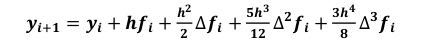
\includegraphics[scale=0.3]{/home/kyoto/workspace/comp_math/VT_labs_2/report/src/img/adams_formula}
\end{figure}

\begin{figure}[H]
    \centering
    где
    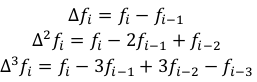
\includegraphics[scale=0.3]{/home/kyoto/workspace/comp_math/VT_labs_2/report/src/img/fki}
\end{figure}
\section{Блок-схема численного метода}
\begin{figure}[H]
    \centering
    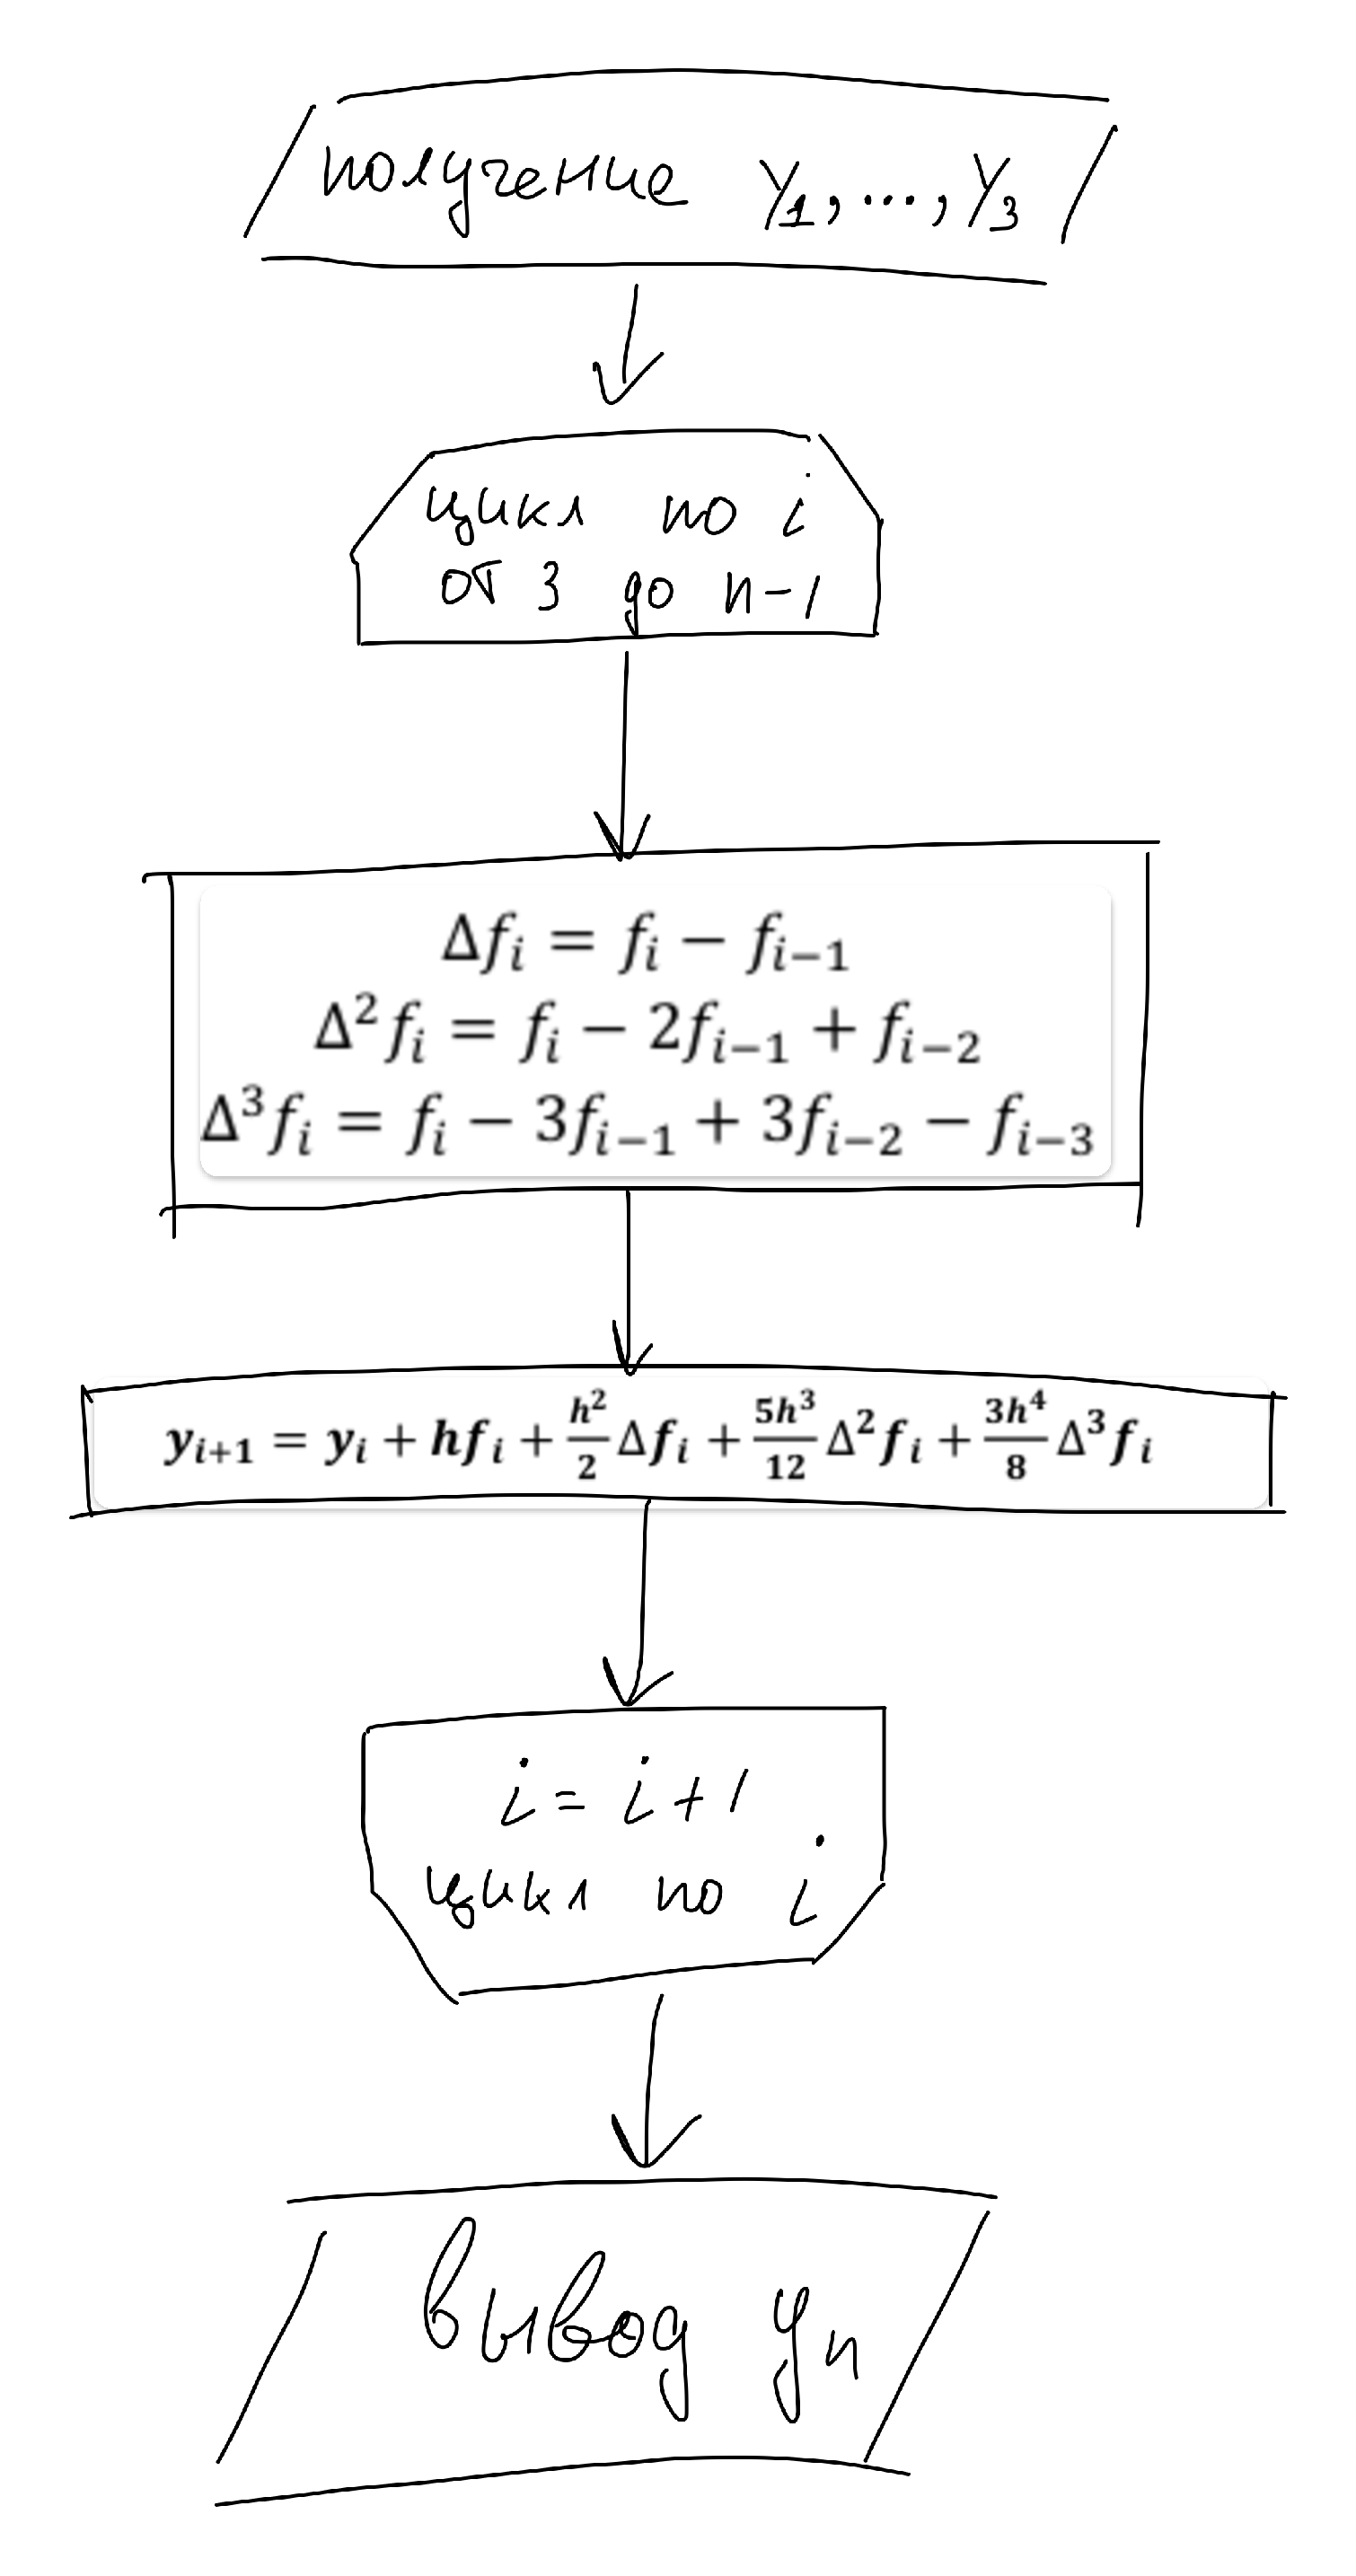
\includegraphics[scale=0.2]{/home/kyoto/workspace/comp_math/VT_labs_2/report/src/img/Untitled 12}
\end{figure}


\section{Listing реализованного численного метода}
\tiny
\begin{verbatim}
    for (int i = 4; i < n; i++) {
        double delta_f_1 = func(X[i], Y[i]);
        double delta_f_2 = func(X[i], Y[i]) - 2 * func(X[i - 1], Y[i - 1]) + func(X[i - 2], Y[i - 2]);
        double delta_f_3 =
                func(X[i], Y[i]) - 3 * func(X[i - 1], Y[i - 1]) + 3 * func(X[i - 2], Y[i - 2]) -
                func(X[i - 3], Y[i - 3]);
        Y[i + 1] = Y[i] + h * func(X[i], Y[i]) + std::pow(h, 2) / 2 * delta_f_1 +
                   std::pow(h, 3) * 5 / 12 * delta_f_2 + std::pow(h, 4) * 3 / 8 * delta_f_3;
    }
    return Y[n];
\end{verbatim}
\normalsize
\newpage

\section{Examples}
\begin{verbatim}
Номер функции: 3
Левая граница: 5
Значение функции y в точке левой границы: 2
Правая граница: 12
\end{verbatim}
\begin{figure}[h]
    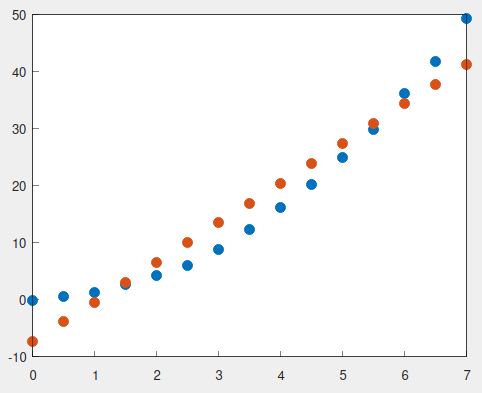
\includegraphics[scale=0.3]{/home/kyoto/workspace/comp_math/VT_labs_2/report/src/img/graphic_1}
\end{figure}


\begin{verbatim}
Номер функции: 2
Левая граница: 1
Значение функции y в точке левой границы: 4
Правая граница: 2
\end{verbatim}
\begin{figure}[h]
    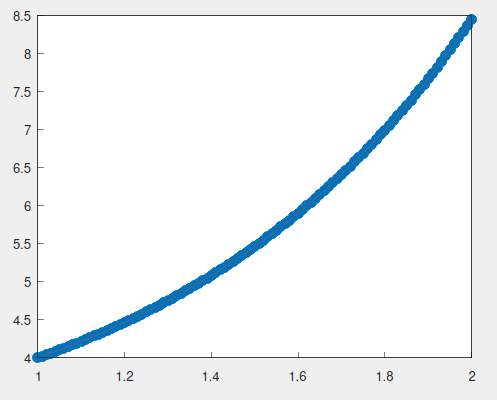
\includegraphics[scale=0.3]{/home/kyoto/workspace/comp_math/VT_labs_2/report/src/img/graphic_2}
\end{figure}

\section{Вывод}
Сравнивая метод Адамса с методом Рунге-Кутта той же точности, отмечаем его экономичность, поскольку он требует вычисления лишь одного значения правой
части на каждом шаге (в методе Рунге-Кутта - четырех). Но метод Адамса неудобен тем, что невозможно начать счет по одному лишь известному значению $y_0$.
Расчет может быть начат только с узла $x_3$, а не $x_0$. Значения $y_1$, $y_2$, $y_3$, необходимые для вычисления $y_4$ нужно получить каким-либо другим
способом (например, методом Рунге-Кутта), что существенно усложняет алгоритм. Кроме того, метод Адамса не позволяет (без усложнения формул) изменить
шаг $h$ в процессе счета -- этого недостатка лишены одношаговые методы.